\documentclass[a4paper,12pt]{article}
\usepackage [utf8x]{inputenc}
\usepackage[czech]{babel} 
\usepackage{graphicx}
\usepackage{amsmath}
\usepackage{xspace}
\usepackage{url}
\usepackage{indentfirst}
\usepackage[margin=22mm]{geometry}
\usepackage{esvect}
\usepackage{ragged2e}
\usepackage{tikz,pgf}
\usepackage{bm}
\usepackage{perpage}
\usepackage{capt-of}
\usepackage{hyperref}
\usepackage{subcaption}
\usepackage{siunitx}

\hypersetup{
	colorlinks=true,
	filecolor=magenta,      
	urlcolor=cyan,
}

\graphicspath{
	{img/}
	{plots/}
	{imgpdf/}
	}

\MakeSorted{figure}
\newtoks\jmenopraktika \newtoks\jmeno \newtoks\datum
\newtoks\obor \newtoks\skupina \newtoks\rocnik \newtoks\semestr
\newtoks\cisloulohy \newtoks\jmenoulohy
\newtoks\tlak \newtoks\teplota \newtoks\vlhkost
\jmenopraktika={Skenovací elektronový mikroskop}  
% nahradte jmenem vaseho predmetu
\jmeno={Radek Horňák}            
\datum={23.~února 2022}        % nahradte datem mereni ulohy
\obor={F}                     
\skupina={Středa 10:00}            
\rocnik={2.}                  
\semestr={IV.}                 
\cisloulohy={6}    % cislo ulohy           

\begin{document}
	\begin{center}
		{\Large Přírodovědecká fakulta Masarykovy univerzity} \\
		\bigskip
		{\Large \bfseries EXPERIMENTÁLNÍ METODY 2} \\
		\bigskip
		{\Large \the\jmenopraktika}
	\end{center}
	\bigskip
	\noindent
	\setlength{\arrayrulewidth}{1pt}
	\begin{tabular*}{\textwidth}{@{\extracolsep{\fill}} l l}
		\large {\bfseries Zpracoval:}  \the\jmeno \hspace{40mm} \large  
		{\bfseries Datum:} \the\datum\\ \\
		\hline
	\end{tabular*}
	
	\section{Úvod}\noindent
Skenovací elektronový mikroskop (SEM) je mikroskop využívající fokusovaný 
paprsek elektronů. Cílem této úlohy je pochopit základní pojmy a principy a 
seznámit se s měřením osobně.
%\par Mezi důležité pojmy SEM je rozlišení spojené s vlnovou délkou, a tedy 
%přímo úměrné energii elektronu.
%\par V teorii jsme se seznámili s důležitými pojmy mikroskopie: rozlišení, 
%optické vady,

\section{Měření}
\subsection{Titanová tříska}\noindent
Prvním měřením bylo sledování povrchu třísky titanu po obrábění. Morfologii 
povrchu vidíme na obrázcích \ref{fig:ti5000}. Snímky byly 
pořízeny při pracovní vzdálenosti (WD) 15,00\,\si{\milli\meter}, urychlovacím 
napětí 6\,\si{\kilo\volt} a zvětšení $500\times$, respektive $5000\times$. 
Vlevo vidíme snímek pořízený SE detektorem, který snímá sekundární elektrony. 
Tyto elektrony jsou generovány z malé hloubky vzorku, typicky několik nanometrů 
a nesou informaci o struktuře povrchu. Na pravé straně je snímek pořízený BSE 
detektorem snímající zpětně odražené elektrony. Pravděpodobnost zpětného 
odražení je úměrná hmotnosti atomu. Tyto snímky nám tedy poskytují informaci o 
rozložení chemických prvků ve vzorku, kde světlejší místa odpovídají těžším 
prvkům. Pro přesnější určení prvků je použita metoda energiově disperzní 
spektroskopie (EDX). Zde detekujeme rentgenové záření emitované ze vzorku. 
Následně z čar charakteristického rentgenového záření jsme schopni určit 
procentuální zastoupení jednotlivých prvků. Tuto analýzu vidíme na 
obr.~\ref{fig:EDX}.  


\begin{figure}[h!]
	\centering
	%\vspace*{-8mm}
	\includegraphics[width=\textwidth]{ti_500x_15mm.pdf}
	\includegraphics[width=\textwidth]{ti_5000x_15mm.pdf}
	%\vspace*{-2mm}
	\caption{\centering }
	\label{fig:ti5000}
\end{figure}


%\begin{figure}[h!]
%	\centering
%	%\vspace*{-8mm}
%	\includegraphics[width=\textwidth]{Electron Image 5.pdf}
%	%\vspace*{-2mm}
%	\caption{\centering }
%	\label{fig:Iab}
%\end{figure}

\begin{figure}[h!]
	\centering
	\begin{subfigure}{0.49\textwidth}
		%\vspace*{-8mm}
		\includegraphics[width=\textwidth]{C Kα1_2 Map Data 5.pdf}
		%\vspace*{-2mm}
		\caption{\centering C K$\alpha_{1,2}$}
		\label{fig:EDX_C}
	\end{subfigure}
	\begin{subfigure}{0.49\textwidth}
		%\vspace*{-8mm}
		\includegraphics[width=\textwidth]{Ti Lα1,2 Map Data 5.pdf}
		%\vspace*{-2mm}
		\caption{\centering Ti L$\alpha_{1,2}$}
		\label{fig:EDX_Ti}
	\end{subfigure}
	\begin{subfigure}{0.49\textwidth}
		%\vspace*{-8mm}
		\includegraphics[width=\textwidth]{O Kα1 Map Data 5.pdf}
		%\vspace*{-2mm}
		\caption{\centering O K$\alpha_{1}$}
		\label{fig:EDX_O}
	\end{subfigure}
	\begin{subfigure}{0.49\textwidth}
		%\vspace*{-8mm}
		\includegraphics[width=\textwidth]{Al Kα1 Map Data 5.pdf}
		%\vspace*{-2mm}
		\caption{\centering Al K$\alpha_{1}$}
		\label{fig:EDX_Al}
	\end{subfigure}
	\label{fig:EDX}
	\caption{Prvkové rozložení ve vzorku určené EDX detektorem.}
\end{figure}

\begin{figure}[h!]
	\centering
	%\vspace*{-8mm}
	\includegraphics[width=\textwidth]{EDS Layered Image 5.pdf}
	%\vspace*{-2mm}

	\begin{subfigure}{0.2\textwidth}
		\vspace*{-60mm}
		\hspace*{65mm}
		
\includegraphics[width=\textwidth]{legend.png}
	\end{subfigure}
	\caption{\centering }
	\label{fig:Iab}
\end{figure}

\begin{figure}[h!]
	\centering
	%\vspace*{-8mm}
	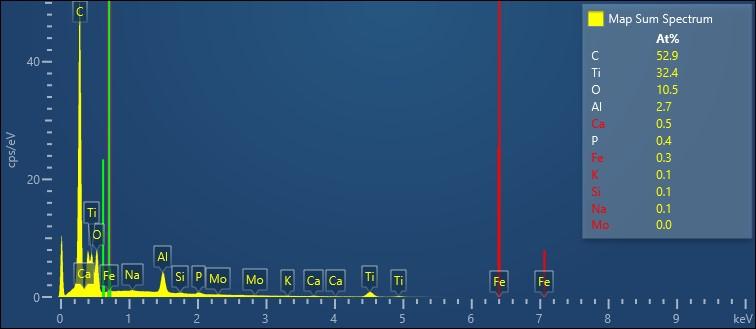
\includegraphics[width=\textwidth]{Map Sum Spectrum.jpeg}
	%\vspace*{-2mm}
	\caption{\centering }
	\label{fig:spectrum}
\end{figure}

\clearpage
\section{Závěr}

	
	
\end{document}
